\chapter{Réalisation}

\section*{Introduction}

\section{Réalisation}
\subsection{Applcation web}
\begin{figure}[H]
    \centering
    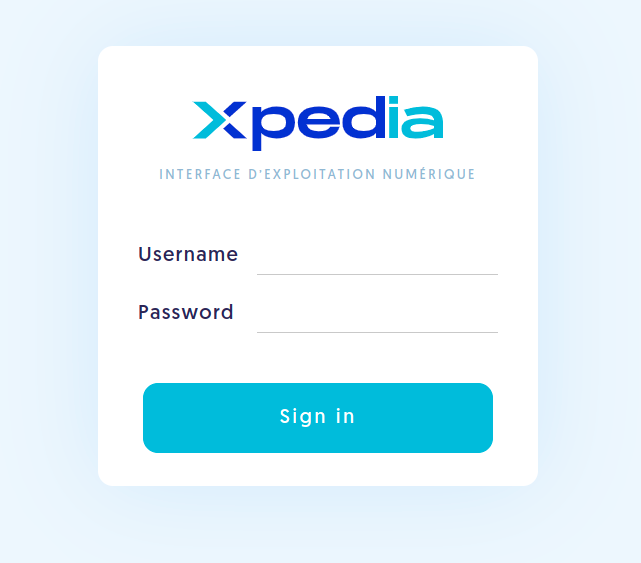
\includegraphics[width=0.8\textwidth]{xpedia_log.png}
    \caption{La login de Xpedia}\label{fig:xpedia_log}
\end{figure}
\begin{figure}[H]
    \centering
    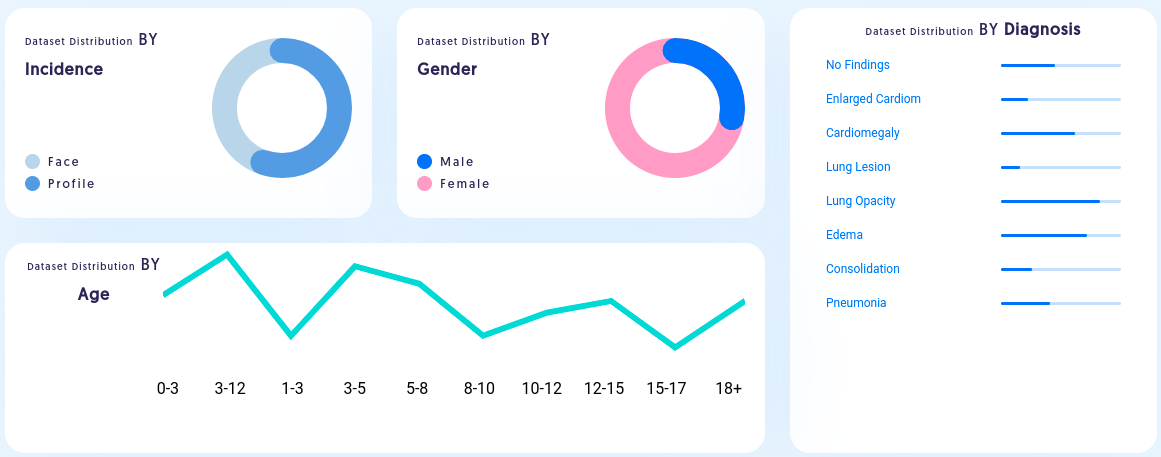
\includegraphics[width=0.8\textwidth]{xpedia_dashboard.png}
    \caption{Le dashboard}\label{fig:xpedia_dashboard}
\end{figure}
\begin{figure}[H]
    \centering
    
\includegraphics[width=0.8\textwidth]{xpedia_menu.png}
    \caption{La menu}\label{fig:xpedia_menu}
\end{figure}
\begin{figure}[H]
    \centering
    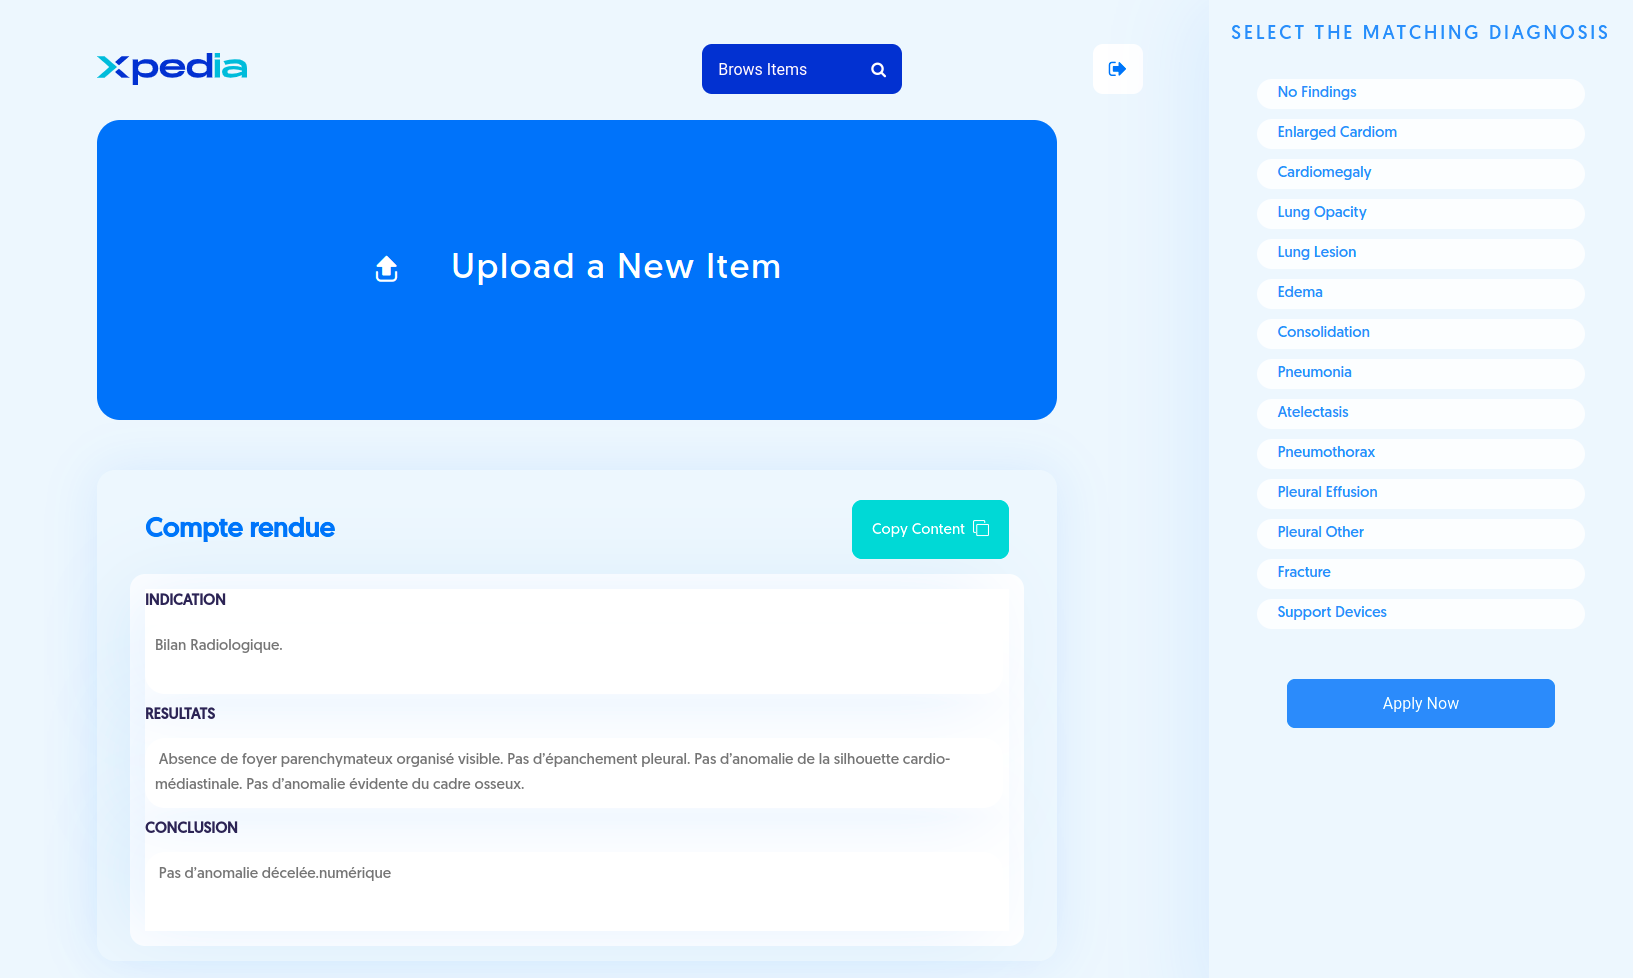
\includegraphics[width=0.8\textwidth]{xpedia_additem.png}
    \caption{La page ajouter élément}\label{fig:xpedia_additem}
\end{figure}
\begin{figure}[H]
    \centering
    
\includegraphics[width=0.8\textwidth]{xpedia_add_image.png}
    \caption{La section réserver à l'jout d'une image}\label{fig:xpedia_add_image}
\end{figure}
\begin{figure}[H]
    \centering
    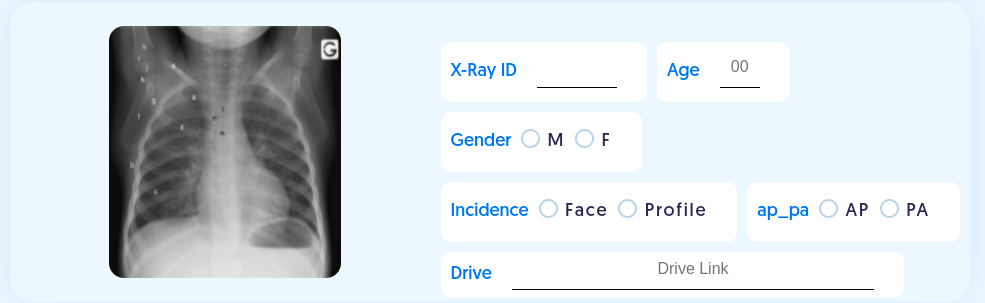
\includegraphics[width=0.8\textwidth]{xpedia_fill_form.png}
    \caption{La formulaire à remplir}\label{fig:xpedia_fill_form}
\end{figure}
\begin{figure}[H]
    \centering
    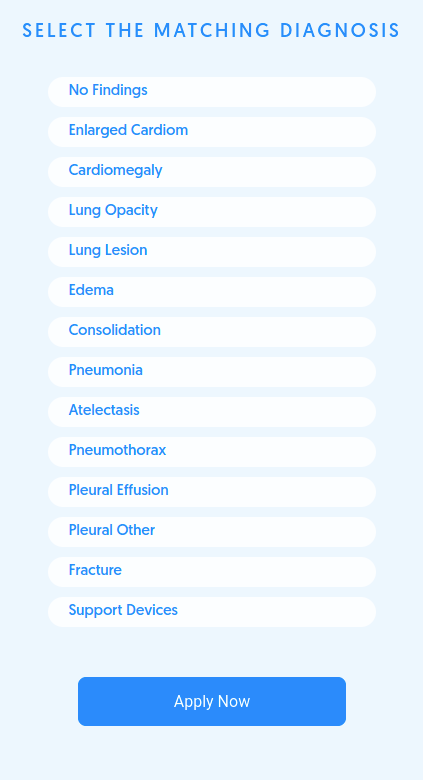
\includegraphics[width=0.8\textwidth]{xpedia_select_section.png}
    \caption{La section de selection des diagnostiques}\label{fig:xpedia_select_section}
\end{figure}
\begin{figure}[H]
    \centering
    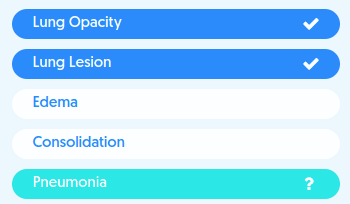
\includegraphics[width=0.8\textwidth]{xpedia_select_items.png}
    \caption{Exemple de selection des diagnostiques}\label{fig:xpedia_select_items}
\end{figure}
\begin{figure}[H]
    \centering
    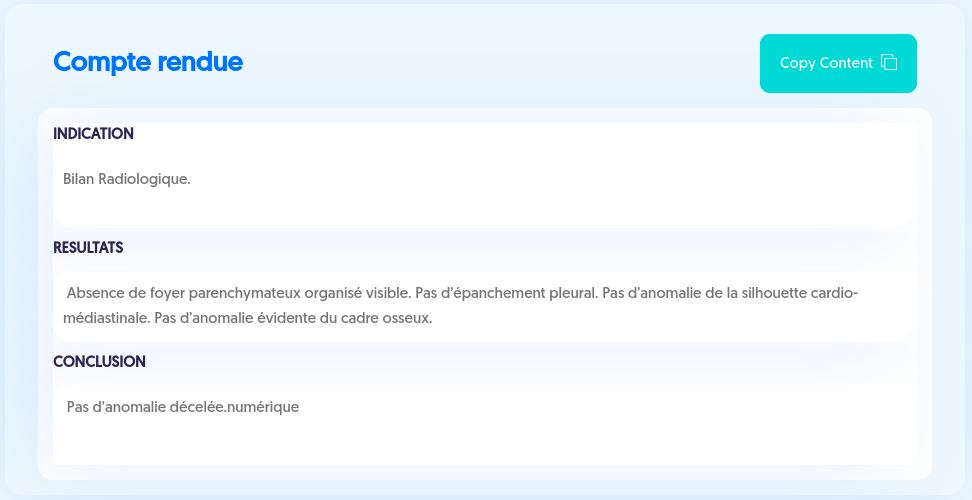
\includegraphics[width=0.8\textwidth]{xpedia_cr}
    \caption{La section du remplissage du compte rendue}\label{fig:xpedia_cr}
\end{figure}
\begin{figure}[H]
    \centering
    
\includegraphics[width=0.8\textwidth]{xpedia_normal_select.png}
    \caption{Choix de 'No Finding' diagnostique}\label{fig:xpedia_menu}
\end{figure}
\begin{figure}[H]
    \centering
    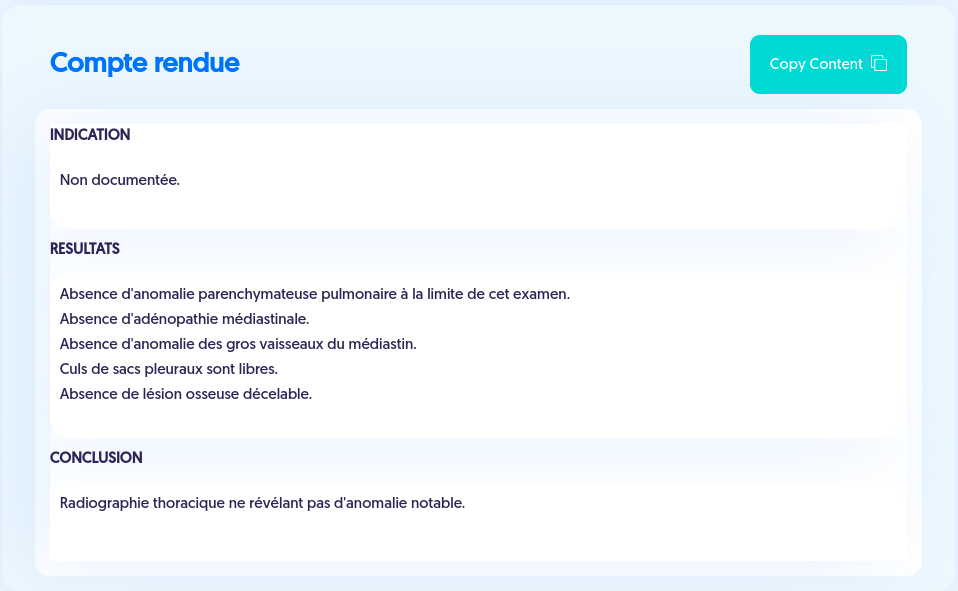
\includegraphics[width=0.8\textwidth]{xpedia_normal_cr.png}
    \caption{Remplissage automatique du compte rendue}\label{fig:xpedia_normal_cr}
\end{figure}
\begin{figure}[H]
    \centering
    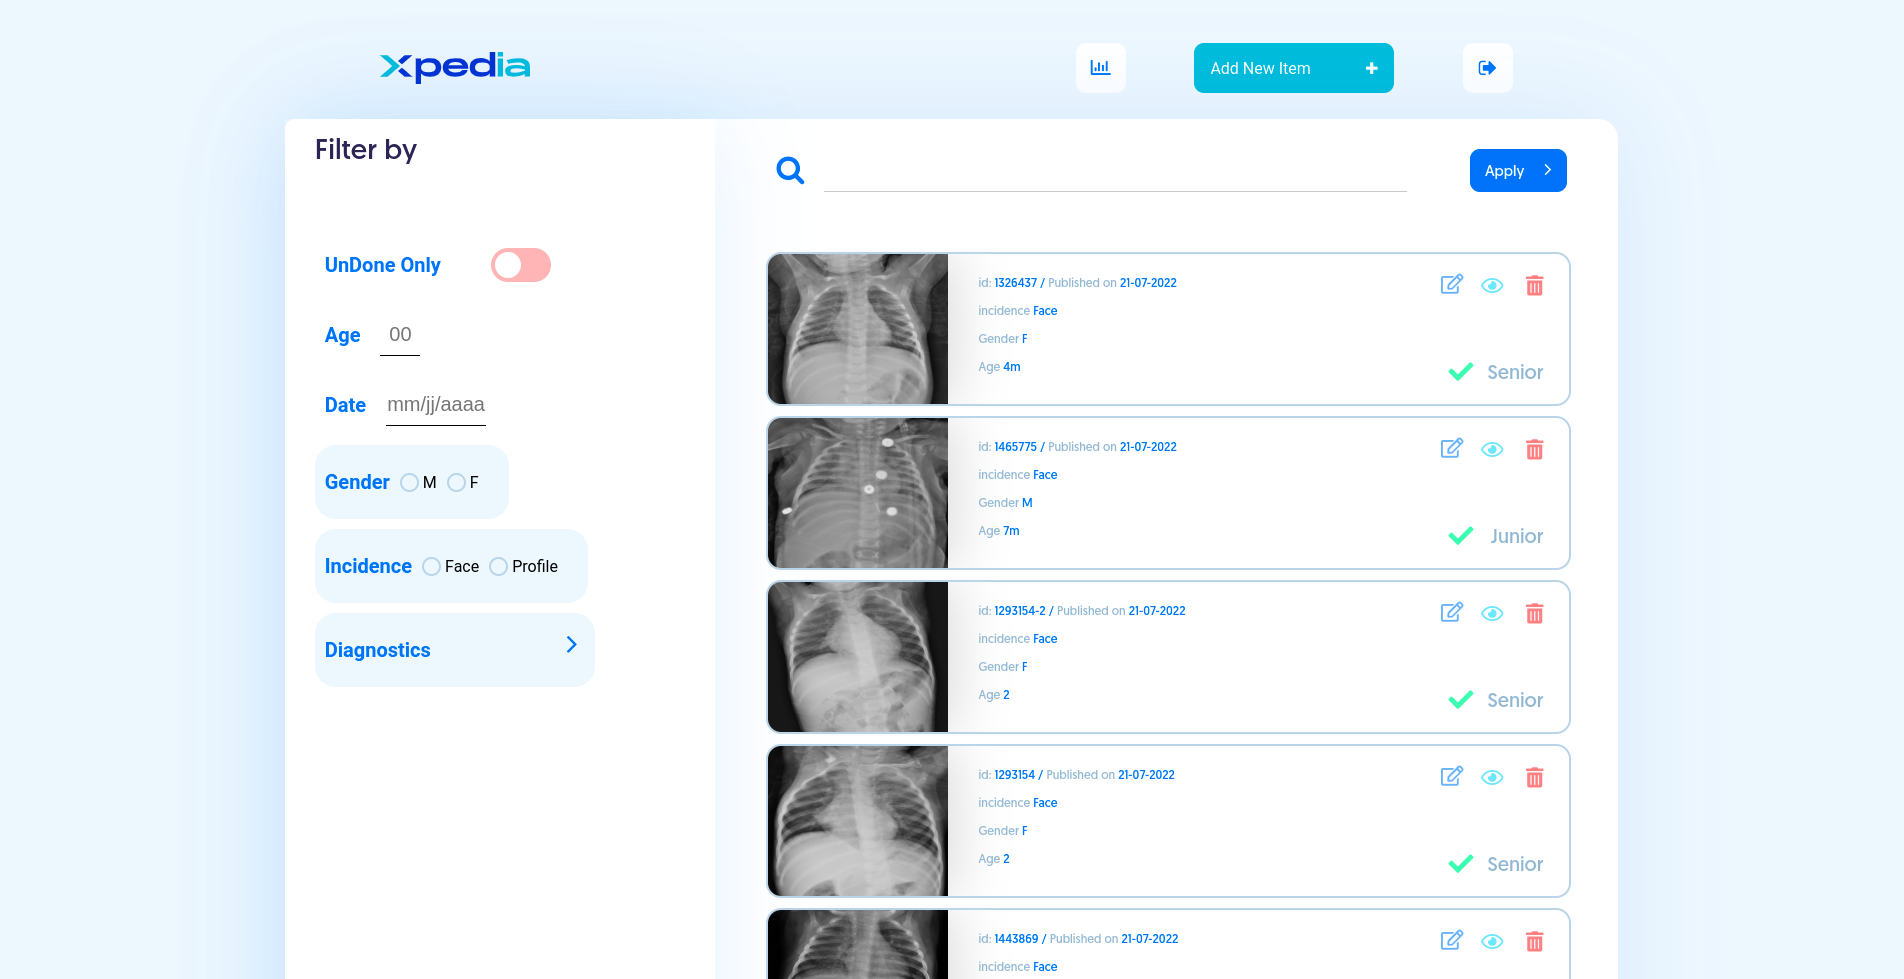
\includegraphics[width=0.8\textwidth]{xpedia_browse_item.png}
    \caption{La page 'browse items'}\label{fig:xpedia_menu}
\end{figure}
\begin{figure}[H]
    \centering
    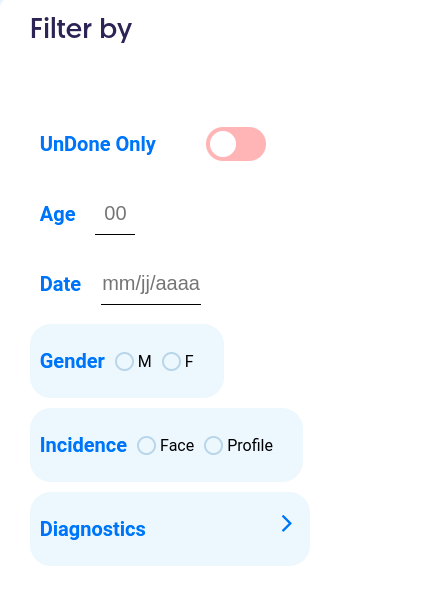
\includegraphics[width=0.8\textwidth]{xpedia_filter_section.png}
    \caption{La section du filtre des éléments}\label{fig:xpedia_filter_section}
\end{figure}
\begin{figure}[H]
    \centering
    
\includegraphics[width=0.8\textwidth]{xpedia_research.png}
    \caption{La bar de recherche}\label{fig:xpedia_research}
\end{figure}
\begin{figure}[H]
    \centering
    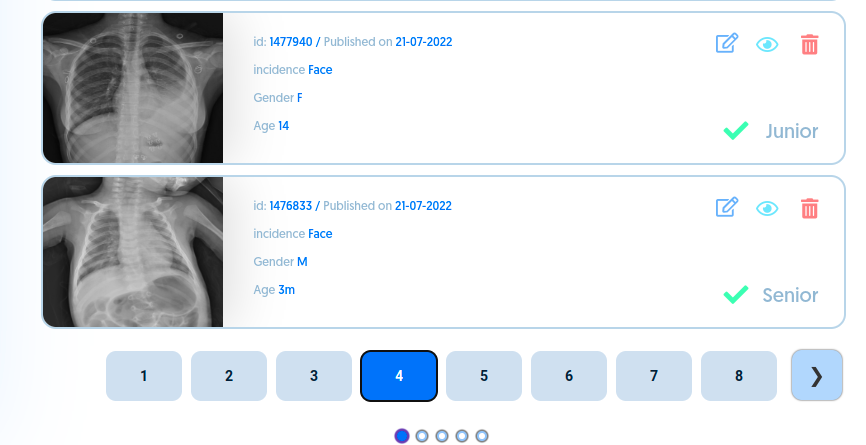
\includegraphics[width=0.8\textwidth]{xpedia_pagination.png}
    \caption{La menu}\label{fig:xpedia_menu}
\end{figure}
\begin{figure}[H]
    \centering
    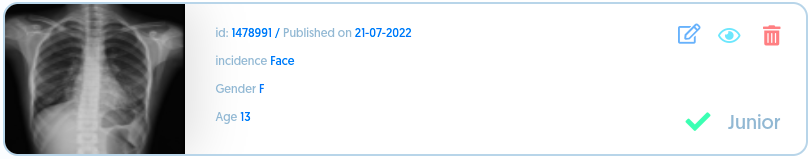
\includegraphics[width=0.8\textwidth]{xpedia_item_thumbnail.png}
    \caption{Vignette de l'élément}\label{fig:xpedia_item_thumbnail}
\end{figure}
\begin{figure}[H]
    \centering
    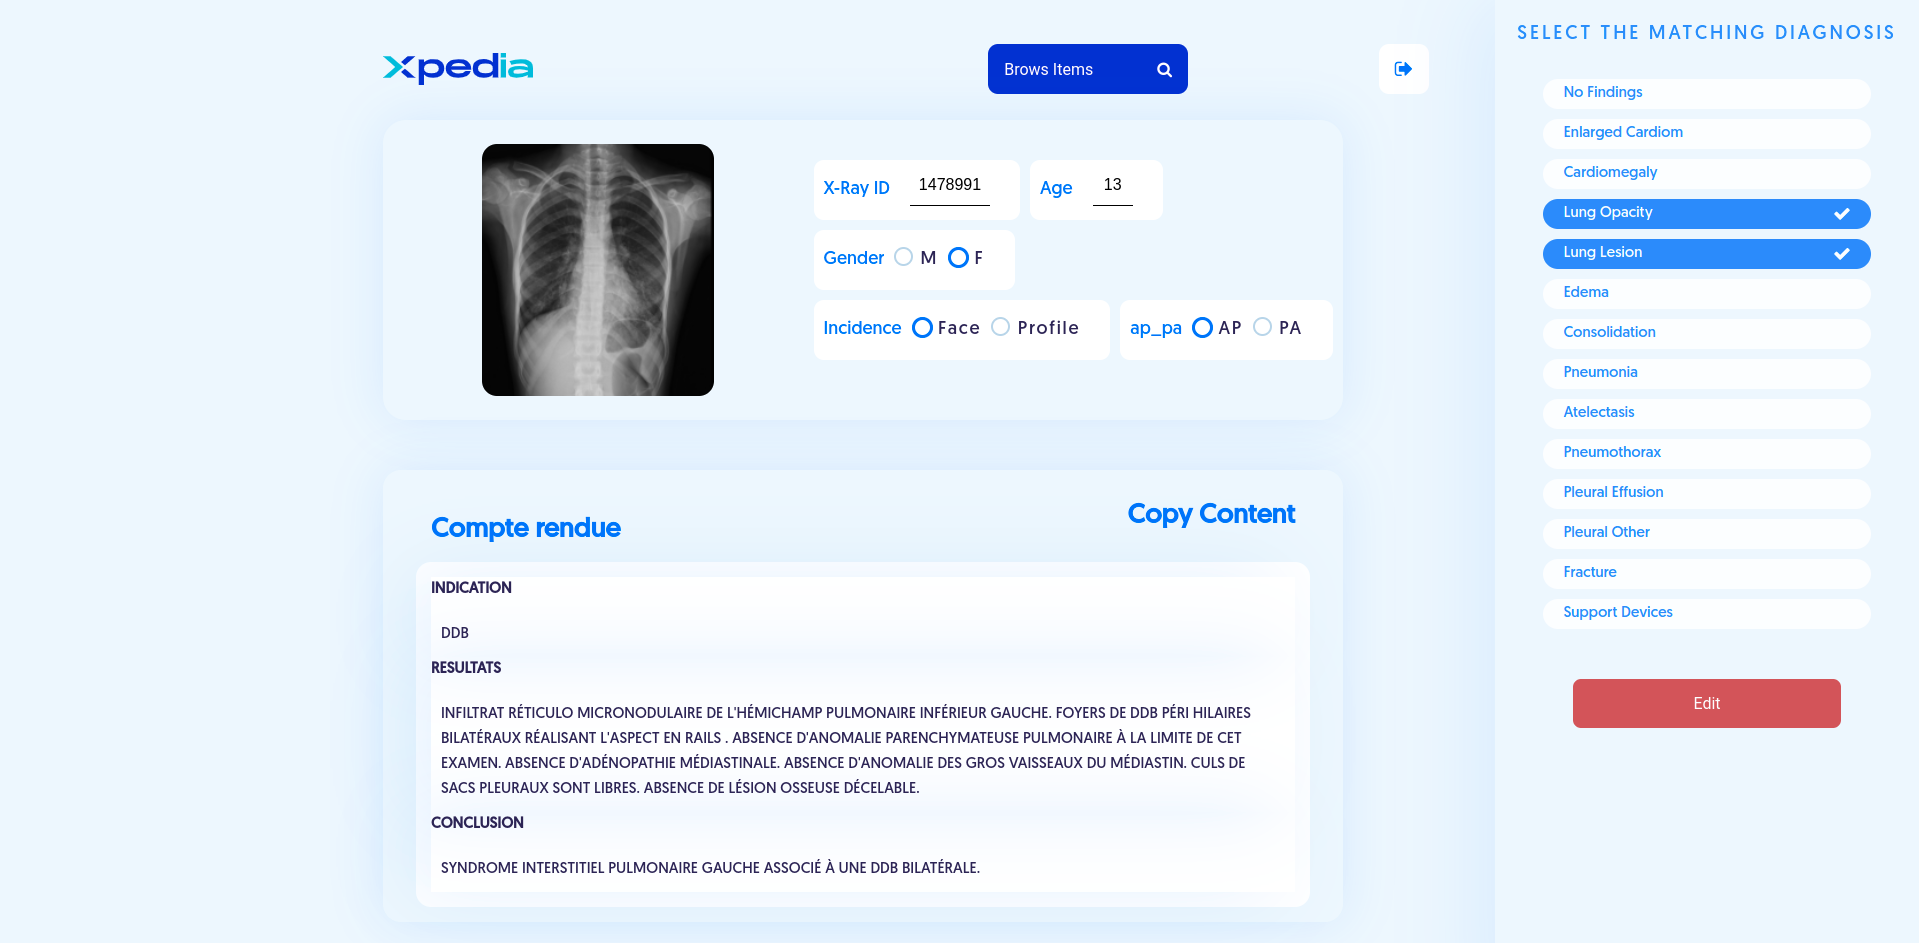
\includegraphics[width=0.8\textwidth]{xpedia_view_page.png}
    \caption{Les détailles de l'élément}\label{fig:xpedia_view_page}
\end{figure}
\begin{figure}[H]
    \centering
    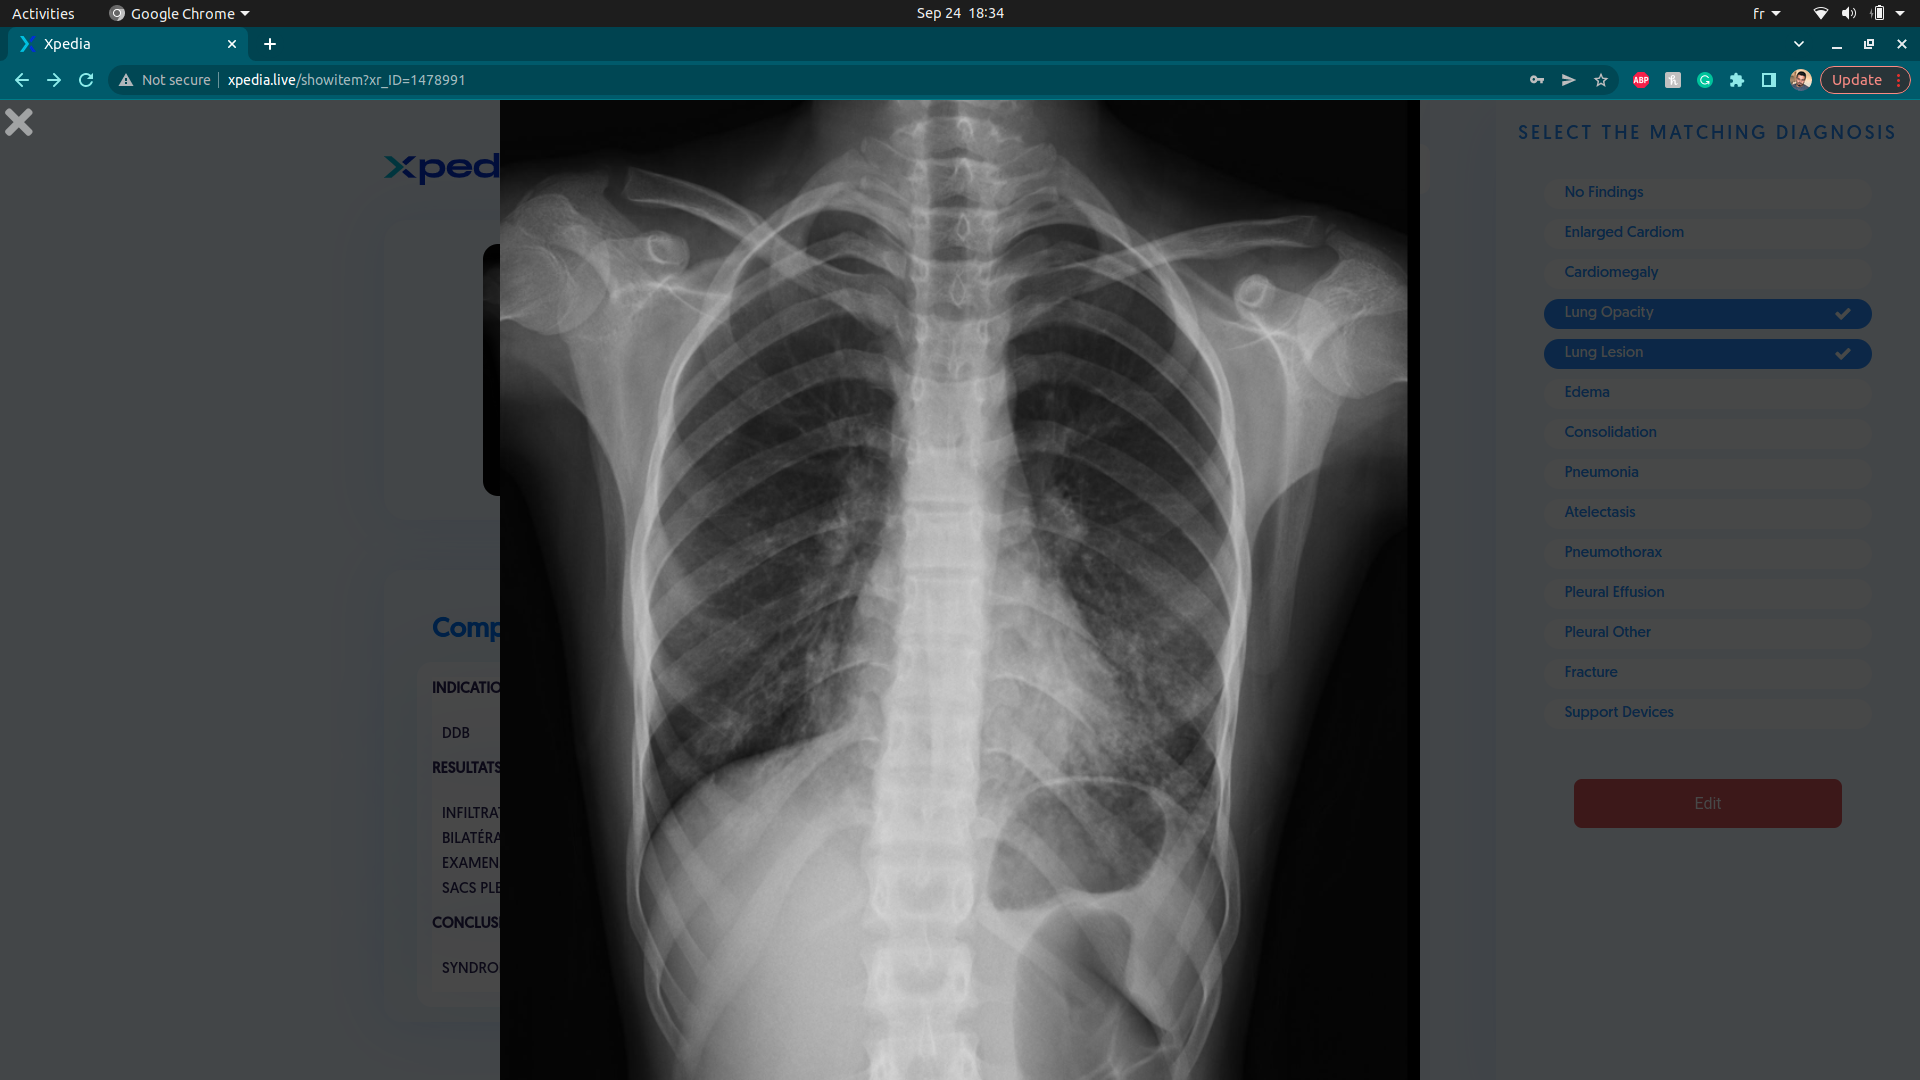
\includegraphics[width=0.8\textwidth]{xpedia_view_showitem.png}
    \caption{Clichés en dimension réel}\label{fig:xpedia_view_showitem}
\end{figure}
\begin{figure}[H]
    \centering
    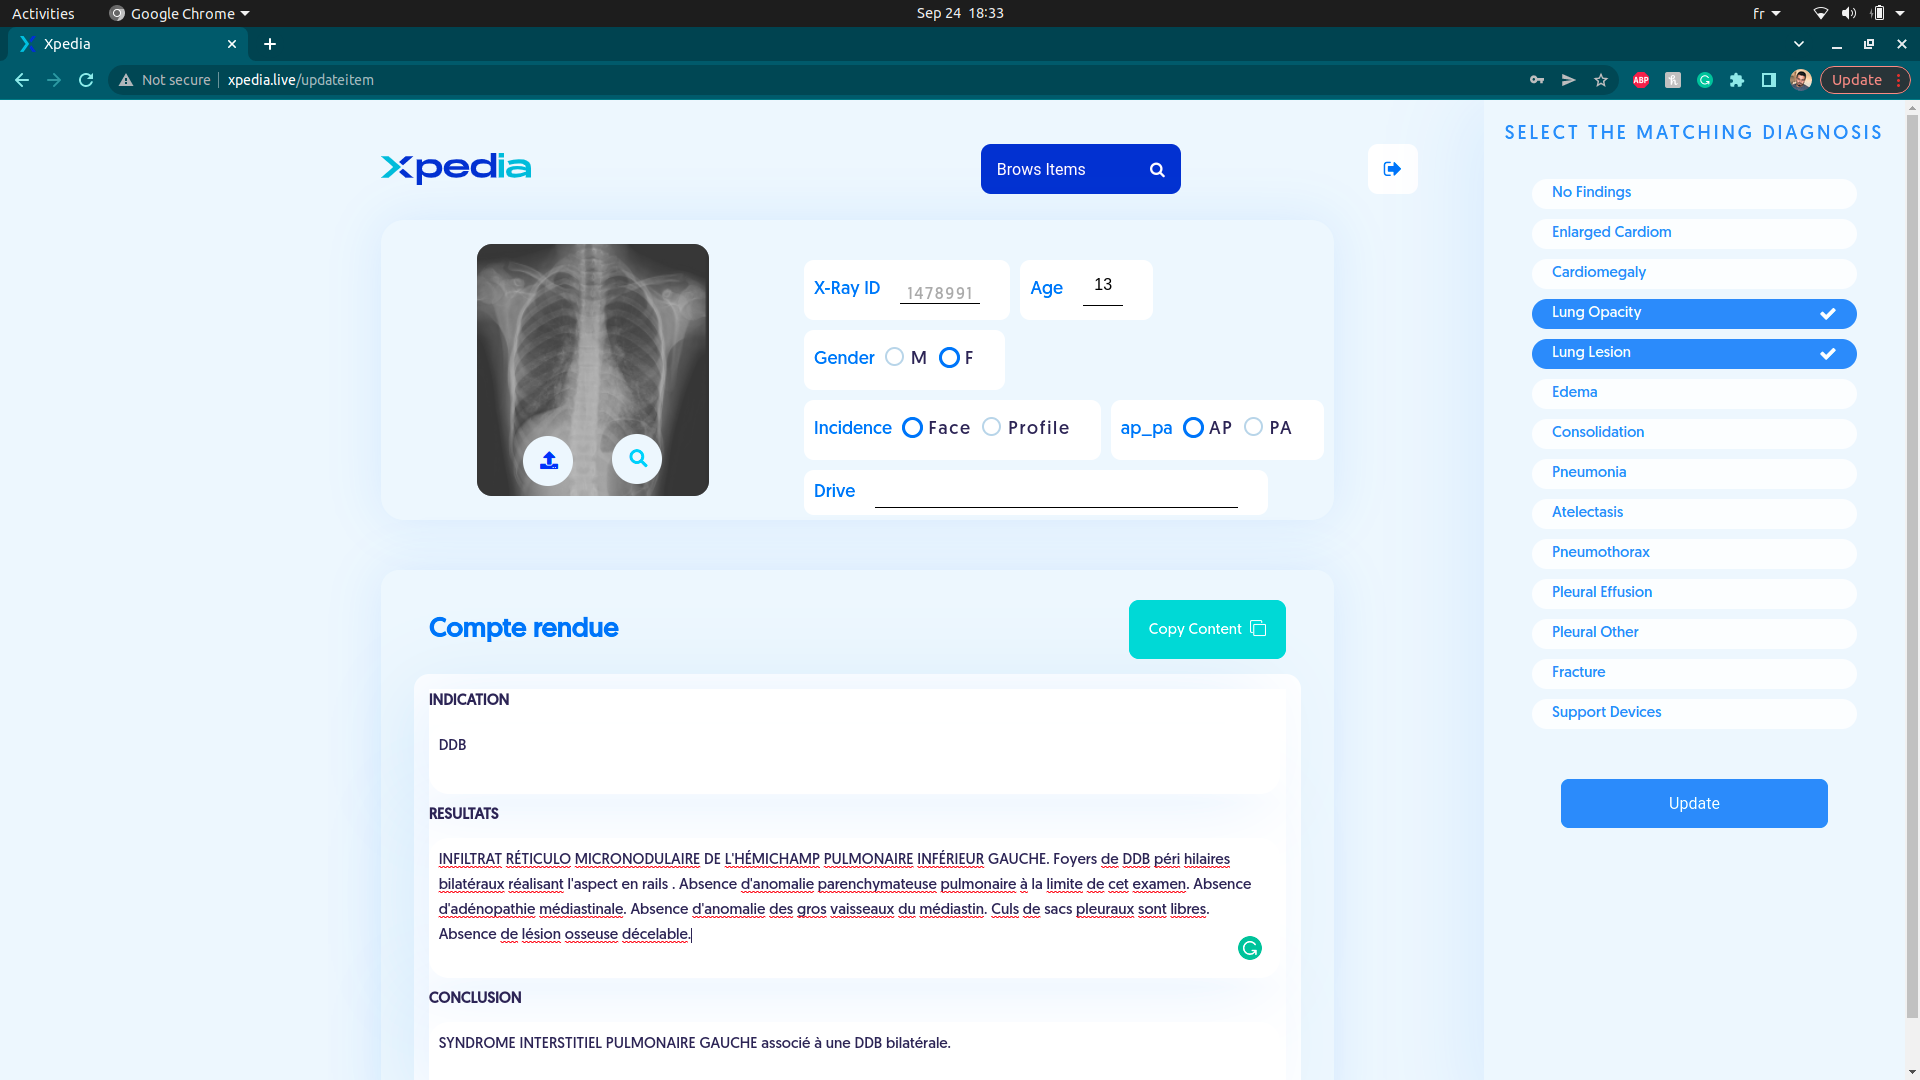
\includegraphics[width=0.8\textwidth]{xpedia_edit_page.png}
    \caption{La page d'edition de l'élément}\label{fig:xpedia_item_thumbnail}
\end{figure}
\subsection{Preparation des données}
\subsection{Madèles d'apprentissage en profondeur}

\section{Experiences}

\section{Résultats}

\section*{Conclusion}